\section{Model}
\label{sec:model}

\setlength{\tabcolsep}{2pt}
\begin{figure*}
\begin{center}
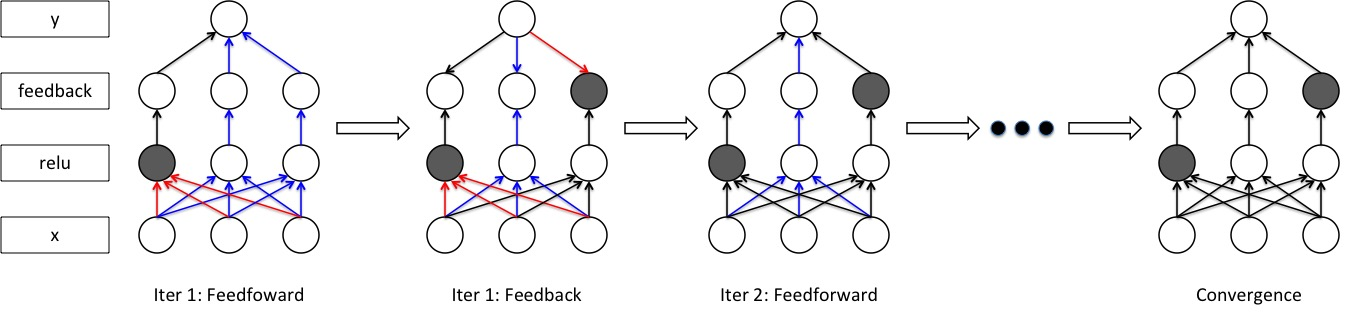
\includegraphics[width=0.95\linewidth]{figs/model/model}
% \vspace{-10pt}
\caption{Illustration of our feedback model and its inference process. At the first iteration, the model performs as a feedforward neural net. After then, the neurons in the feedback hidden layers update their activation status to maximize the confidence output of the target top neuron. This process continues until convergence. (We show only one layer here, but the feedback layers can be tacked in the deep ConvNet.) Better viewed in color.}
\label{fig:model}
% \vspace{-30pt}
\end{center}
\end{figure*}

We first review the current state-of-the-art feedforward Deep Convolutional Neural Networks (CNNs) architecture and then propose our feedback model on top of that. 

\subsection{Review of Convolutional Neural Networks}
The most recent state-of-the-art deep CNNs~\cite{Simonyan2014Very} consist of many stacked feedforward layers, including convolutional, rectified linear units (ReLU) and max-pooling layers. For each layer, the input $\mathbf{x}$ can be an image or the output of a previous layer, consisting of $C$ input channels of width $M$ and height $N$: $\mathbf{x} \in \mathcal{R}^{M \times N \times C}$. The output $\mathbf{y}$ consists of a set of $C'$ output channels of width $M'$ and height $N'$: $\mathbf{y} \in \mathcal{R}^{M' \times N' \times C'}$. 

\textbf{Convolutional Layer:} 
The convolutional layer is parameterized by $C'$ filters with every filter $\mathbf{k} \in \mathcal{R}^{K \times K \times C}$.
\begin{equation}
\mathbf{y}_{c'} = \sum_{c=1}^C \mathbf{k}_{c'c} * \mathbf{x}_c
\end{equation}

\textbf{ReLU Layer:}
The ReLU layer is used to provide the nonlinearity for the network.
\begin{equation}
\mathbf{y} = \max (\mathbf{0}, \mathbf{x})
\end{equation} 

\textbf{Max-Pooling Layer:}
The max-pooling layer is used to reduce the dimensionality of the output and model the invariance in deformable objects. The max-pooling operation is usually applied over a small neighborhood $\mathcal{N}$ for every pixel location $i,j$ in the image.
\begin{equation}
y_{i,j,c} = \max_{u,v \in \mathcal{N}} x_{i+u, j+v, c}
\end{equation}

\begin{comment}
\textbf{Fully Connnected Layer:} The fully connected layer is parameterized by the production matrix with $W \in \mathcal{R}^{M'N'C' \times MNC}$. 
Finally, a few fully connected layers (normally with drop-out) is stacked on top of the convolutional outputs to compute the scores of every class. 
\begin{equation}
\vec{y}_l = W_l^T  \vec{y}_{l-1}
\end{equation}
\end{comment}

\subsection{Re-interpretion of ReLU and Max-Pooling}
In the ConvNet, each output of the convolutional layer is forward as the input of ReLU layer. In the architeture, low-level convolutional filters tend to learn biologically plausible feature detectors, such as Gabor filters, while filers in higher layers learn to respond to concrete visual objects or their parts. The ReLU neurons control the activation of the filtering results, to make sure the useful low-level information (above 0) is passed and irrelavent information is stopped.

We model the max function as neuron activation gates $h$ with binary values 0 or 1. For the ReLU layer, the gates work as turn on the neuron to let the below message pass or turn off the neuron to stop the message flow. For the Max-Pooling layer, the gates work similarly as ReLU, except only one gate can be open among a local region.

For the ReLU layer, 
\begin{equation}
y_l(i,j,c) = h_l(i,j,c) \cdot y_{l-1}(i,j,c)
\end{equation} 
where $h_l(i,j,c) = 0$ when $y_{l-1}(i,j,c) <= 0$ and $h_l(i,j,c) = 1$ when $y_{l-1}(i,j,c) > 0$.

For the max-pooling layer,
\begin{equation}
y_l(i,j,c) = \sum_{} h_l(u, v) \cdot y_{l-1}(i+u, j+v, c)
\end{equation}

\subsection{Hidden Neuron Activations in Feedback}
However, in order to recognize the image, the middle level layers are designed to provide all possible information for the final layer to classify. This works well when there is only one salient object in the image. However when people care about different aspects in the images, the same feature may not be appropriate all the time. 

Since the model open all the gates for the gates for all information to pass, when we are targeted on a paticular semantic labels, we want to turn off those gates that provide irrelavant information for seeing that object. This top-down message will be utilized to turn off those relu.

We model the top down as another type of activation variable, similar as ReLu. However, this unit activates based on the the overall information of bottom-up responses and top-down messages. 

To understand the model, we allow each ReLU neuron to either turn on, turn off, or pass a proportion of the information computed from the convolutional layer, in order to maximially interpret the image as the target class.

We model a feedback layer on top of the relu layers to improve the activation felxibility, that the feedback neuron activation variables depend on the weights from high level targets. When combined with ReLU layer, the two layers not only capture on the bottom-up features but also top-down weights passed from the target neuron. Figure.~\ref{fig:model} illustrates the architecture of our model and the inference process. 
 
Given an image $I$ and a neural network with learned parameters $w$, we optimize the target neuron output by jointly reasoning neuron activiations $h$ over all the hidden layers. Particularly, if the target neuron is the class node in the top layer, we optimize the class score $S_c$ by looking for the reorganization of hidden neuron activations on the ReLU layer:
\begin{equation}
\begin{aligned}
  \max_h S_c(I_0, h) \\
  s.t.\ h_i \in \{0, 1\}
\end{aligned}
\end{equation}

This leads to an integer programming problem, which is a NP-hard problem given the current deep convolutional neural net structure. To obtain a good solution, we apply a linear relaxation.

In the linear relaxation, we rephrase the problem as:
\begin{equation}
\begin{aligned}
  \max_h S_c(I_0, h) \\
  s.t.\ 0 \leq h_i \leq 1
\end{aligned}
\end{equation}

\begin{comment}
To understand the model, we allow each ReLU neuron to either turn on, turn off, or pass a proportion of the information computed from the convolutional layer, in order to maximially interpret the image as the target class.

We use the gradient descent method to optimize $h$. After convergence we discretize $h$ to 0 or 1.

In practice, we treat the inference process as discriminatively optimize the final class node. 

Optimizing such function results in an integer programming, if we treat h as binary variables. 

During optimization, we proposed two ways to deal with it, 1. coordinate descent 2. continuous relaxation

Hard optimization: The coordinate descent frameworks stand in this way: 1. Initialize h as all 1 meaning the gate is open, compute feedfoward messages to the class node, then given the current activation status, optimize the last layer h to maximize the class output, given the updates last layer h, keep optimizing lower layers. And reiterate this process.

Soft optimization: The continuous relaxation falls in below way, compute the gradient of class node y given h, use gradient descent update h, and keep until this until convergence.
\end{comment}

\subsection{Relationship to the Deconvolutional Neural Networks}


To understand how our inference algorithm work exactly, we compare it to the Deconvolutional neural networks model~\cite{}.

we show below, DeconvNet-based reconstruction of the n-th layer input Xn is either equivalent or similar to computing the gradient of the visualised neuron ac-tivity f with respect to Xn, so DeconvNet effectively corresponds to the gradient back-propagation through a ConvNet.

We can conclude that apart from the RELU layer, computing the approximate feature map recon- struction Rn using a DeconvNet is equivalent to computing the derivative ∂f/∂Xn using back- propagation, which is a part of our visualisation algorithms. Thus, gradient-based visualisation can be seen as the generalisation of that of [13], since the gradient-based techniques can be applied to the visualisation of activities in any layer, not just a convolutional one. In particular, in this paper we visualised the class score neurons in the final fully-connected layer.

Following this, deconvnet can be viewed as a one iteration of our hard optimization

\subsection{Implementation Details}


